\documentclass{scrartcl}
\KOMAoptions{parskip=half}

\usepackage{amssymb}
\usepackage{amsmath}
\usepackage{amsthm}

\usepackage{tikz}
\usetikzlibrary{quotes}

\theoremstyle{definition}
\newtheorem{definition}{Definition}

\theoremstyle{plain}
\newtheorem{conjecture}{Conjecture}
\newtheorem{corollary}{Corollary}
\newtheorem{lemma}{Lemma}
\newtheorem{theorem}{Theorem}

\usepackage{caption} % make figure hyperref link to correct place.
\setlength\intextsep{\textfloatsep} % set desired figure spacing.

\usepackage{hyperref}

\title{Exploring Barnette's Conjecture}
\author{Steven Xia}
\date{December 6, 2023}

\begin{document}
\maketitle

\section*{Terminology}

We will assume knowledge of basic graph theoretic terminology, with all graphs being finite, simple
and undirected.
Define a \textit{Barnette graph} to be a bipartite 3-connected cubic planar graph.
Let a graph be \textit{Hamiltonian} if it contains a Hamiltonian cycle.
Then we state the main focus of this paper as such:

\begin{conjecture}[Barnette's conjecture]
    Every Barnette graph is Hamiltonian.
\end{conjecture}

Define the \textit{length} of a face $f$ in a plane graph to be the number of edges incident to
that face, and denote this value by $\lvert f\rvert$.
Call a face \textit{small} if it is of length 4, and \textit{big} otherwise.
For all other terminology, we refer to \cite{Diestel2017-lj}.

\section*{Introduction}

In 1884, Tait \cite{Tait1884-zt} conjectured that every 3-connected cubic planar graph is
Hamiltonian.
A proof of this would have been a major breakthrough, since it implies the four colour theorem.
However, Tutte \cite{Tutte1946-mn} disproved the conjecture in 1946 by constructing a
counterexample.
Tutte \cite{Tutte1971-rb} then conjectured that every bipartite 3-connected cubic graph is
Hamiltonian, but this was also disproven by a counterexample published in \cite{Bondy1976-db}.

Barnette's conjecture \cite{Tutte1969-mj} was first published in 1969, and is the intersection of
the two above conjectures.
We note that the above counterexamples imply the conditions of bipartiteness and planarity are
required for the conjecture to hold.
In fact, it can be shown (with examples) that 3-connectedness and cubicity are also required.
This means that if the conjecture were to be true, it would be a ``tight'' classification of
Hamiltonian graphs.
We also know \cite{Tutte1956-dq} that 4-connected planar graphs are Hamiltonian, so Barnette's
conjecture lies on the thin line between Hamiltonian and non-Hamiltonian planar graphs.
This paper will survey the literature surrounding the conjecture along with illustrate of some
elementary attempts at proving related results.

\section*{Survey of known results}

Over fifty years after its publication, Barnette's conjecture is still open with no consensus on
whether it is true.
In this section, we provide results directly supporting the conjecture as well as a plethora of
equivalent formulations.

\subsection*{Partial results}

Soon after Barnette stated his conjecture, Goodey \cite{Goodey1975-sz} verified it for Barnette
graphs with short faces, showing the following results:

\begin{theorem}
    Every Barnette graph with every face having length 4 or 6 is Hamiltonian.
\end{theorem}

\begin{theorem}
    Every Barnette graph with one face of length 8 and every other face having length 4 or 6 is
    Hamiltonian.
\end{theorem}

We note that the two sets of graphs referenced by Goodey's theorems can be described succinctly as
Barnette graphs with at most seven small faces.
This equivalence can be shown as follows:

\begin{proof}
    Let $G$ be a Barnette graph with $v$ vertices, $e$ edges, and $f$ faces.
    Since $G$ is connected and planar, Euler's formula gives $v-e+f=2$.
    But $G$ is also cubic, so actually $v-\frac{3v}2+f=2$, which gives $f=\frac{1}2v+2$.

    Also since $G$ is cubic, we have
    $$\sum_{k\in F(G)}\lvert k\rvert=3v\iff \sum_{k\in F(G)}\left(\lvert k\rvert-6\right)=3v-6f=-12\text{.}$$
    Since all faces of length less than 6 are of length 4, this shows that every Barnette graph
    must have at least 6 faces of length 4.
    Furthermore, every face $k$ of length more than 4 corresponds to $(\lvert k\rvert-6)/2$ faces
    of length 4.
\end{proof}

This reframing does not improve any results but may facilitate certain proof approaches.
For example, we can try to extend Goodey's results to eight small faces, using the fact that
decreasing the number of small faces instantly solves the problem.

On the topic of Goodey's proofs, it was shown in \cite{Holton1985-yo} that every Barnette graph can
be generated by starting at the cube graph and applying the operations in Figure
\ref{fig:vertex operation} and Figure \ref{fig:edge operation} (hereinafter, the
\textit{vertex operation} and the \textit{edge operation} respectively).
Actually, we see that every Hamiltonian cycle can be extended through the vertex operation, and
that almost every configuration in which a Hamiltonian cycle can pass around edges $e$ and $f$ (in
Figure \ref{fig:edge operation}) can be extended through the edge operation.
Indeed, the only case in which a Hamiltonian cycle cannot be extended is if both edges $e$ and $f$
are avoided in the original Hamiltonian cycle.
Reframing Goodey's proofs this way, the casework in their proofs mainly dealt with this scenario,
and used the restriction of the face lengths to provide some framework to exhaustively work through
all the cases.
Once we loosen the restriction by allowing two faces of length 8, the number of cases increases
drastically, which is perhaps why there has not been any improvements to Goodey's partial results
using similar induction arguments.

\begin{figure}
    \centering

    \begin{tikzpicture}[
            nodes={draw, circle, fill=black, inner sep=0, minimum size=5pt},
            label distance=1pt]
        \node (1) [label={30:$v$}] at (0,0) {};
        \path (1) ++( 90:15mm) edge (1);
        \path (1) ++(210:15mm) edge (1);
        \path (1) ++(330:15mm) edge (1);

        \draw [->, very thick] (3.5,0) -- (4.5,0);

        \node (a) [label=$v$] at (8,0) {};
        \path (a) ++( 30: 7mm) node (b) {};
        \path (a) ++( 90:10mm) node (c) {};
        \path (a) ++(150: 7mm) node (d) {};
        \path (a) ++(210:10mm) node (e) {};
        \path (a) ++(270: 7mm) node (f) {};
        \path (a) ++(330:10mm) node (g) {};
        \draw (a) -- (b) -- (c) -- (d);
        \draw (a) -- (d) -- (e) -- (f);
        \draw (a) -- (f) -- (g) -- (b);
        \path (c) ++( 90:5mm) edge (c);
        \path (e) ++(210:5mm) edge (e);
        \path (g) ++(330:5mm) edge (g);
    \end{tikzpicture}
    \caption{Vertex operation on vertex $v$}
    \label{fig:vertex operation}
\end{figure}

\begin{figure}
    \centering
    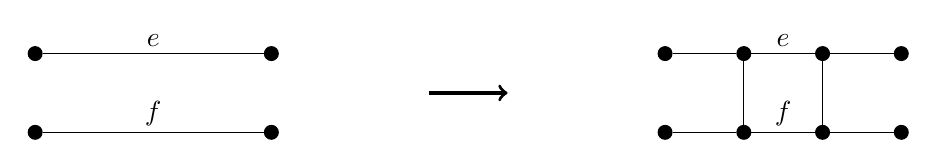
\begin{tikzpicture}[nodes={draw, circle, fill=black, inner sep=0, minimum size=5pt}]
        \node (1) at (0,1) {};
        \node (2) [right of=1, node distance=3cm] {} edge ["$e$"{above, inner sep=1pt, draw=none, fill=white, fill opacity=0, text opacity=1}] (1);
        \node (3) [below of=1] {};
        \node (4) [right of=3, node distance=3cm] {} edge ["$f$"{above, inner sep=1pt, draw=none, fill=white, fill opacity=0, text opacity=1}] (3);

        \draw [->, very thick] (5,0.5) -- (6,0.5);

        \node (a) at (8,1) {};
        \node (b) [right of=a] {} edge (a);
        \node (c) [right of=b] {} edge ["$e$"{above, inner sep=1pt, draw=none, fill opacity=0, text opacity=1}] (b);
        \node (d) [right of=c] {} edge (c);
        \node (e) [below of=a] {};
        \node (f) [right of=e] {} edge (e);
        \node (g) [right of=f] {} edge ["$f$"{above, inner sep=1pt, draw=none, fill opacity=0, text opacity=1}] (f);
        \node (h) [right of=g] {} edge (g);
        \draw (b) -- (f);
        \draw (c) -- (g);
    \end{tikzpicture}
    \caption{Edge operation on edges $e$ and $f$}
    \label{fig:edge operation}
\end{figure}

In fact, all recent results surrounding Barnette's conjecture have been achieved by translating the
problem into different formulations.
For example, using an equivalence \cite{Stein1971-zh} between the Hamiltonicity of a Barnette graph
and the existence of an induced tree in its dual graph satisfying a particular condition, Florek
\cite{Florek2010-un} showed the following:

\begin{theorem}
    Every Barnette graph containing a 2-factor in which every component is a facial 4-cycle is
    Hamiltonian.
\end{theorem}

It is known \cite{Konig1916-fe} that every Barnette graph has a 3-edge-colouring, so therefore has
at least three distinct 2-factors.
That is to say it is not too outlandish to be restricting Barnette graphs based on their 2-factors.
All other recent results proceed this way: transform Barnette's conjecture into a different
problem, often on the dual graph, then proceed from there.
These cannot be described concisely, so an interested reader can find them at
\cite{Bagheri_Gh2021-ic} and \cite{Florek2016-ip}, with a not yet published paper at
\cite{Florek2023-vw}.

We end this section by stating that computational efforts \cite{Brinkmann2021-eb} have verified
Barnette's conjecture for graphs on at most 90 vertices.
However, since the minimal counterexample for Tait's conjecture \cite{Holton1988-qm} (Barnette's
without bipartiteness) is on 38 vertices and the minimal counterexample for Tutte's conjecture
\cite{Brinkmann2021-eb} (Barnette's without planarity) is on 50 vertices, it is expected for any
minimal counterexample to Barnette's conjecture to be large.
Furthermore, it was also shown \cite{Bagheri_Gh2022-xk} that if Barnette's conjecture is false,
then deciding whether a Barnette graph is Hamiltonian is NP-complete.

\subsection*{Equivalent forms}

In order to better understand Barnette's conjecture, some equivalent statements have been proven.
Many of these strengthen the conjecture, hoping to allow easier construction of a possible
counterexample.
The most prominant of these results was shown by Kelmans in \cite{Kelmans1994-qp}\footnotemark{}
and states the following:

\footnotetext{Actually, Kelmans showed this earlier and the citation is an English translation of
              the proof.}

\begin{theorem}
    \label{thm:kelmans1994}
    Barnette's conjecture holds if and only if for every Barnette graph $G$ and a pair of edges
    $e,f\in E(G)$ incident to a same face, there exists a Hamiltonian cycle passing through $e$ but
    avoiding $f$.
\end{theorem}

The proof is by a clever construction of a larger Barnette graph in which the existence Hamiltonian
cycle would imply a Hamiltonian cycle in the original graph with the desired properties.
The two edges being on the same face is necessary for the construction to work, so loosening that
restriction using the same argument is impossible.
That being said, if a Hamiltonian cycle avoids some edge of a face of a Barnette graph, this means
it must include the two edges adjacent (in the facial cycle) to the missing edge, thus Theorem
\ref{thm:kelmans1994} implies we can inculde any two arbitrary edges incident to a face in a
Hamiltonian cycle.
On the other hand, we know that we cannot always avoid two arbitrary edges incident to a face.
For example, let $G$ be the graph of a hexagonal prism and let $e_1,\dots,e_6$ be the edges of
a facial cycle of length 6, and we see that $G$ has no Hmiltonian cycle avoiding both edges $e_1$
and $e_4$.

Kelmans' result was used by Hertel \cite{hertel2005} to prove the following strengthening:

\begin{theorem}
    Barnette's conjecture holds if and only if for every Barnette graph $G$ and a path
    $P\subseteq G$ of length 3, there exists a Hamiltonian cycle containing $P$.
\end{theorem}

Similarly to above, we note that this result cannot be improved to work with arbitrary paths of
length 4. For example, the Barnette graph in Figure \ref{fig:path of length 4} does not contain a
Hamiltonian cycle containing the thick edges.

\begin{figure}[h]
    \centering

    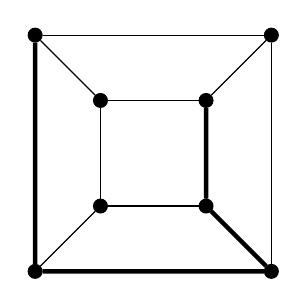
\begin{tikzpicture}[
            nodes={draw, circle, fill=black, inner sep=0, minimum size=5pt},
            node distance=1.173cm]
        \node (1) at (0,1) {};
        \node (2) [right of=1, node distance=3cm] {};
        \node (3) [above of=2, node distance=3cm] {};
        \node (4) [left of=3, node distance=3cm] {};
        \draw (1) -- (2) -- (3) -- (4) -- (1);

        \node (5) [above right of=1] {} edge (1);
        \node (6) [above left of=2] {} edge (2);
        \node (7) [below left of=3] {} edge (3);
        \node (8) [below right of=4] {} edge (4);
        \draw (5) -- (6) -- (7) -- (8) -- (5);

        \draw [ultra thick] (4) -- (1) -- (2) -- (6) -- (7);
    \end{tikzpicture}
    \caption{Path of length 4 not in a Hamiltonian cycle}
    \label{fig:path of length 4}
\end{figure}

On the other hand, Harant \cite{Harant2013-nn} showed a seemingly much weaker statement of
Barnette's conjecture, which goes as follows:

\begin{theorem}
    Barnette's conjecture holds if and only if there exists a constant $c>0$ such that every
    Barnette graph has a path of length $c\lvert V(G)\rvert$.
\end{theorem}

This was proved by showing that if Barnette's conjecture were false, we can construct an infinite
sequence of non-Hamiltonian Barnette graphs where, in the limit, the fraction of vertices in the
longest cycle goes to 0.
By a result by Bondy and Locke \cite{Bondy1981-lt}, this would imply there is also no path of
similar length.
The construction in this proof highlights one of the main issues when working on Barnette's
conjecture.
Since they are planar, Barnette graphs lack global structure, but are also not connected enough or
dense enough to easily force long cycles.

\section*{Attempted proofs and other work}

This section will describe two approches in which tangible results were found.

\subsection*{Possible weakening of Barnette's conjecture}

Here, we try to state a weakening of Barnette's conjecture.
In particular, we show that if for every Barnette graph $G$ there exists a fixed construction which
splits an arbitrary face $k\in F(G)$ of $G$ in half to form another Barnette graph $G^\prime$ in
such a way that Hamiltonicity of $G^\prime$ implies Hamiltonicity of $G$, then there exists a
constant $c$ such that  Barnette's conjecture holds if and only if every Barnette graph with faces
of length at most $c$ has a Hamiltonian cycle.
In this case, a \textit{fixed construction} is one which can be applied to any face of sufficient
length, and only introduces a constant number of faces of constant length as well as possibly
increasing the lengths of a constant number of existing faces by a constant amount.
Let $C$ be the facial cycle of $k$ in $G$ and we will abuse notation (for this section) to let $k$
denote both the face as well as the number of edges incident to $k$.
Then a construction \textit{splitting a face in half} means that we allow the area in $G^\prime$
corresponding to the area bounded by $C$ in $G$ to contain two faces of size $ak+b$ and $(1-a)k+b$
respectively, for constants $0<a<1$ and $b\in\mathbb{N}$.

To elaborate, consider a face $k\in F(G)$ and let $C$ be the facial cycle of $k$ which has edge
sequence $e_1,\dots,e_k$.
Set $e=e_1$ and $f\in\{e_{k/2},e_{k/2+1}\}$ to be edges which are of odd index in $C$, so $e$ and
$f$ are separated by an odd number of edges in $C$ (both ways).
Now apply the edge operation (in Figure \ref{fig:edge operation}) to edges $e$ and $f$ to create
$G^\prime$.
Clearly, this is a fixed construction: it introduces one new face of length 4 and increases the
lengths of two faces by 2.
Note that this construction also splits $k$ into halves.
However, we do not know that every Hamiltonian cycle in $G^\prime$ can be brought back to $G$.
Indeed, if a Hamiltonian cycle takes exactly one of the two ``vertical'' edges (in Figure
\ref{fig:edge operation}) in $G^\prime$, we cannot trivially construct a Hamiltonian cycle in $G$.
Therefore, this construction would not generate a weakening of Barnette's conjecture.
Now we can actually state and prove our initial statement.

\begin{theorem}
    If there exists a fixed construction which can be applied to any Barnette graph $G$ to split
    any face (of sufficient length) in half and create a new Barnette in which Hamiltonicity
    implies the Hamiltonicity of $G$, then there exists a constant $c$ for which Barnette's
    conjecture holds if and only if every Barnette graph with faces of length at most $c$ is
    Hamiltonian.
\end{theorem}

\begin{proof}
    Suppose there exists a construction satisfying the conditions of the hypothesis.
    Let $G$ be a Barnette graph and we will show that there exists a constant $c$ for which
    repeatedly applying the construction to a longest face of $G$ a finite number of times will
    result in a graph which has all faces of length at most $c$.

    Let $\mathcal{B}$ be the class of Barnette graphs and define $s:\mathcal{B}\to \mathbb{N}$ to
    be $s(G)=\sum_{f\in F(G)}f^2$.
    Suppose $k\in F(G)$ is a longest face so applying the construction to $k$ splits it into two
    faces of lengths at most $ak+b$ and $(1-a)k+b$ respectively, for constants $0<a<1$ and
    $b\in\mathbb{N}$, while increasing the lengths of faces $f_1,\dots,f_p\in F(G)$ by
    $g_1,\dots,g_p\in\mathbb{N}$ and adding faces $h_1,\dots,h_q$.
    Let $G^\prime$ be the new graph, and see that
    \begin{align*}
        s(G^\prime)<s(G)
        &\iff (ak+b)^2+((1-a)k+b)^2+\sum_{i=1}^p(f_i+g_i)^2+\sum_{j=1}^qh_i^2<k^2+\sum_{i=1}^pf_i^2 \\
        &\iff 2a(a-1)k^2+2bk+\sum_{i=1}^p2f_ig_i+\left(2b^2+\sum_{i=1}^pg_i^2+\sum_{j=1}^qh_i^2\right)<0
    \end{align*}
    Now since $k\geq f_i$ for all $1\leq i\leq p$, the above inequality is implied by
    \begin{align*}
        \phantom{-----}
        &\impliedby 2a(a-1)k^2+2bk+\sum_{i=1}^p2kg_i+\left(2b^2+\sum_{i=1}^pg_i^2+\sum_{j=1}^qh_i^2\right)<0 \\
        &\iff 2a(a-1)k^2+\left(2b+\sum_{i=1}^p 2g_i\right)k+\left(2b^2+\sum_{i=1}^pg_i^2+\sum_{j=1}^qh_i^2\right)<0
    \end{align*}
    Now since $0<a<1\implies 2a(a-1)<0$, the left hand side of the above inequality is a
    polynomial in $k$ with constant coefficients and a negative leading coefficient, which means
    there exists a constant $c$ for which the inequality holds for all $k>c$.

    From here, set $G_0=G$ and consider the sequence of graphs $G_0,G_1,G_2,\dots$ where $G_{i+1}$
    is generated by applying the construction to a longest face of $G_i$.
    Let $G_d$ be the first graph in the sequence for which $s(G_{d+1})\geq s(G_d)$, which we know
    exists because $s$ is an integer valued function which is bounded below by $0$.
    But this means the longest face of $G_d$ is of length less than $c$.
    We denote the graph $G_d$ as $t(G)$.
    
    To finish the proof, we show the equivalence.
    If Barnette's conjecture is true, then clearly every Barnette graph with faces of length at
    most $c$ is Hamiltonian.
    Conversely, if every Barnette graph with faces of length at most $c$ is Hamiltonian, then for
    every Barnette graph $G$ with a face of length more than $c$, we can bring a Hamiltonian cycle
    in $t(G)$ back to a Hamiltonian cycle in $G$.
\end{proof}

We comment that all fixed constructions are close to being Barnette graphs themselves.
For example, if we took the two opposing edges $e$ and $f$ of a longest cycle (as in the first
example) and applied the edge operation twice, we would have a construction which can be easily
ripped out of the original graph and turned into a standalone Barnette graph (in this case, the
cube graph) just by connecting the vertices of degree less than 3.
Then the problem of whether a construction forces a Hamiltonian cycle in the generated graph to be
able to be brought back to the original graph can be viewed as whether this Barnette graph cannot
have certain sets of paths which partition the vertices, and results helping with this may come
naturally from efforts to generate counterexamples.

\begin{figure}[h]
    \centering
    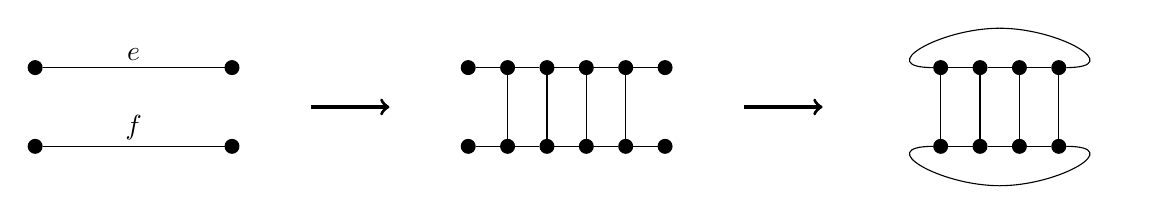
\begin{tikzpicture}[
            nodes={draw, circle, fill=black, inner sep=0, minimum size=5pt},
            node distance=5mm]
        \node (1) at (0,1) {};
        \node (2) [right of=1, node distance=25mm] {} edge ["$e$"{above, inner sep=1pt, draw=none, fill=white, fill opacity=0, text opacity=1}] (1);
        \node (3) [below of=1, node distance=1cm] {};
        \node (4) [right of=3, node distance=25mm] {} edge ["$f$"{above, inner sep=1pt, draw=none, fill=white, fill opacity=0, text opacity=1}] (3);

        \draw [->, very thick] (3.5,0.5) -- (4.5,0.5);

        \node (a) at (5.5,1) {};
        \node (b) [right of=a] {} edge (a);
        \node (c) [right of=b] {} edge (b);
        \node (d) [right of=c] {} edge (c);
        \node (e) [right of=d] {} edge (d);
        \node (f) [right of=e] {} edge (e);
        \node (A) [below of=a, node distance=1cm] {};
        \node (B) [right of=A] {} edge (A);
        \node (C) [right of=B] {} edge (B);
        \node (D) [right of=C] {} edge (C);
        \node (E) [right of=D] {} edge (D);
        \node (F) [right of=E] {} edge (E);
        \draw (b) -- (B);
        \draw (c) -- (C);
        \draw (d) -- (D);
        \draw (e) -- (E);

        \draw [->, very thick] (9,0.5) -- (10,0.5);

        \node (b) at (11.5,1) {};
        \node (c) [right of=b] {} edge (b);
        \node (d) [right of=c] {} edge (c);
        \node (e) [right of=d] {} edge (d);
        \node (B) [below of=b, node distance=1cm] {};
        \node (C) [right of=B] {} edge (B);
        \node (D) [right of=C] {} edge (C);
        \node (E) [right of=D] {} edge (D);
        \draw (b) -- (B);
        \draw (c) -- (C);
        \draw (d) -- (D);
        \draw (e) -- (E);

        \path (12.25,1.5) edge [out=180, in=180, looseness=2] (b);
        \path (12.25,1.5) edge [out=  0, in=  0, looseness=2] (e);
        \path (12.25,-0.5) edge [out=180, in=180, looseness=2] (B);
        \path (12.25,-0.5) edge [out=  0, in=  0, looseness=2] (E);
    \end{tikzpicture}
    \caption{Turning a valid construction to a Barnette graph}
    \label{fig:cube construction}
\end{figure}

% \subsection*{Long cycles in the double graphs of special Barnette graphs}
%
% In this final section, we prove a partial result on the double graphs of Barnette graphs.
% The \textit{double graph}\footnotemark{} of a graph $G$ is created by copying $G$, mapping vertex
% $v_i$ in $G$ to $u_i$ in the copy of $G$, then adding edges $v_iu_i$ for every $i$.
% For example, under this definition we can realize the $(d+1)$-dimensional cube as the double graph
% the $d$-dimensional cube. 
%
% \footnotetext{This definition is different than what is common in literature because this
%               particular construction was not found to be referenced anywhere.
%               Maybe it is not interesting... }

\subsection*{Making Barnette graphs Hamiltonian}

In this final section, we describe a construction which can modify any Barnette graph to make
it Hamiltonian.
Unfortunately, this construction is destructive in the sense that the new graph is not a Barnette
graph, so the result does not seem particularly useful.
However, it does show that graphs with few big faces have long paths.

\begin{theorem}
    Every Barnette graph can be made Hamiltonian by adding at most one edge to each of its big
    faces.
\end{theorem}

\begin{proof}
    Let $G$ be a Barnette graph.
    As long as there exists a vertex $v$ which is incident to three small faces, we can apply the
    inverse of the vertex operation (in Figure \ref{fig:vertex operation}) to $v$.
    If eventually there still exists a vertex incident to three small faces but we cannot apply the
    inverse of the vertex operation, then we have the cube graph which is Hamiltonian, in which
    case a Hamiltonian cycle can be extended to a Hamiltonian cycle of $G$.
    Therefore, we may assume this process terminates at a graph $G^\prime$ which does not have any
    vertices which are incident to three small faces.

    For every big face of $G^\prime$, add a vertex in that face with edges connecting to every
    vertex incident to that face to create $G^{\prime\prime}$, which we claim is 4-connected.
    For a contradiction, suppose there exists a separating set of three vertices.
    It is easy to see that every such separating set must have vertices of $V(G^\prime)$ on both
    sides of the separation.
    This means if a vertex of the separating set is in $V(G^{\prime\prime})\setminus V(G^\prime)$,
    then the remaining two vertices would form a 2-separation of $G^\prime$, a contradiction.
    Therefore, we may assume all three vertices of the separating set are in $V(G^\prime)$, and it
    suffices to show that every 3-separation in $G^\prime$ has a big face which is incident to both
    sides of the separation.
    We will show this by case work.
    \begin{figure}[hb]
        \centering
        \begin{minipage}{0.33\textwidth}
            \centering
            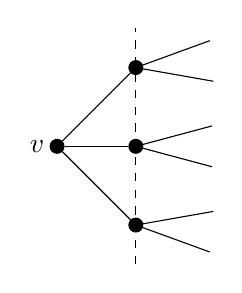
\begin{tikzpicture}[
                    nodes={draw, circle, fill=black, inner sep=0, minimum size=5pt},
                    label distance=1pt]
                \node (2) at (0,2) {};
                \node (1) at (0,1) {};
                \node (0) at (0,0) {};
                \draw [dashed] (0,-0.5) -- (0,2.5);

                \node (3) [label={180:$v$}] at (-1,1) {};
                \draw (3) -- (2);
                \draw (3) -- (1);
                \draw (3) -- (0);

                \path (2) ++( 20:1cm) edge (2);
                \path (2) ++(-10:1cm) edge (2);
                \path (1) ++( 15:1cm) edge (1);
                \path (1) ++(-15:1cm) edge (1);
                \path (0) ++( 10:1cm) edge (0);
                \path (0) ++(-20:1cm) edge (0);
            \end{tikzpicture}
            \caption{}
            \label{fig:lemma case 1}
        \end{minipage}
        \hfill
        \begin{minipage}{0.33\textwidth}
            \centering
            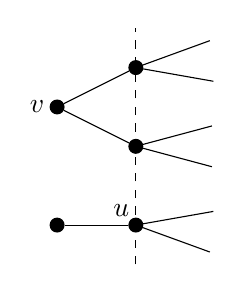
\begin{tikzpicture}[
                    nodes={draw, circle, fill=black, inner sep=0, minimum size=5pt},
                    label distance=1pt]
                \node (2) at (0,2) {};
                \node (1) at (0,1) {};
                \node (0) [label={135:$u$}] at (0,0) {};
                \draw [dashed] (0,-0.5) -- (0,2.5);

                \node (3) [label={180:$v$}] at (-1,1.5) {};
                \draw (3) -- (2);
                \draw (3) -- (1);
                \path (0) ++(180:1cm) node (_) {} edge (0);

                \path (2) ++( 20:1cm) edge (2);
                \path (2) ++(-10:1cm) edge (2);
                \path (1) ++( 15:1cm) edge (1);
                \path (1) ++(-15:1cm) edge (1);
                \path (0) ++( 10:1cm) edge (0);
                \path (0) ++(-20:1cm) edge (0);
            \end{tikzpicture}
            \caption{}
            \label{fig:lemma case 2}
        \end{minipage}
        \hfill
        \begin{minipage}{0.32\textwidth}
            \centering
            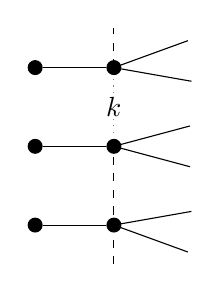
\begin{tikzpicture}[nodes={draw, circle, fill=black, inner sep=0, minimum size=5pt}]
                \node (2) at (0,2) {};
                \node (1) at (0,1) {};
                \node (0) at (0,0) {};
                \draw [dashed] (0,-0.5) -- (0,1);
                \draw [dotted, opacity=0.5] (0,1) -- (0,2);
                \draw [dashed] (0,2) -- (0,2.5);
                \node (_) [draw=none, fill=white] at (0,1.5) {$k$};

                \path (2) ++(180:1cm) node (_) {} edge (2);
                \path (1) ++(180:1cm) node (_) {} edge (1);
                \path (0) ++(180:1cm) node (_) {} edge (0);

                \path (2) ++( 20:1cm) edge (2);
                \path (2) ++(-10:1cm) edge (2);
                \path (1) ++( 15:1cm) edge (1);
                \path (1) ++(-15:1cm) edge (1);
                \path (0) ++( 10:1cm) edge (0);
                \path (0) ++(-20:1cm) edge (0);
            \end{tikzpicture}
            \caption{}
            \label{fig:lemma case 3}
        \end{minipage}
    \end{figure}
    First suppose at most six of the edges incident to the separation is to one side, then we have
    one of three cases: if we have Figure \ref{fig:lemma case 1}, then by construction we know that
    one of the faces incident to $v$ is a big face; if we have Figure \ref{fig:lemma case 2}, then
    $\{u,v\}$ forms a 2-separation of $G^\prime$, a contradiction; and if we have Figure
    \ref{fig:lemma case 3}, then the face $k$ is a big face.
    \begin{figure}[hb]
        \centering
        \begin{minipage}{0.33\textwidth}
            \centering
            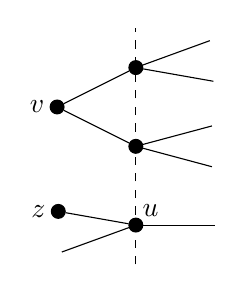
\begin{tikzpicture}[
                    nodes={draw, circle, fill=black, inner sep=0, minimum size=5pt},
                    label distance=1pt]
                \node (2) at (0,2) {};
                \node (1) at (0,1) {};
                \node (0) [label={45:$u$}] at (0,0) {};
                \draw [dashed] (0,-0.5) -- (0,2.5);

                \node (3) [label={180:$v$}] at (-1,1.5) {};
                \draw (3) -- (2);
                \draw (3) -- (1);
                \path (0) ++(170:1cm) node [label={180:$z$}] (_) {} edge (0);
                \path (0) ++(200:1cm) edge (0);

                \path (2) ++( 20:1cm) edge (2);
                \path (2) ++(-10:1cm) edge (2);
                \path (1) ++( 15:1cm) edge (1);
                \path (1) ++(-15:1cm) edge (1);
                \path (0) ++(  0:1cm) edge (0);
            \end{tikzpicture}
            \caption{}
            \label{fig:lemma case 4}
        \end{minipage}
        \hfill
        \begin{minipage}{0.33\textwidth}
            \centering
            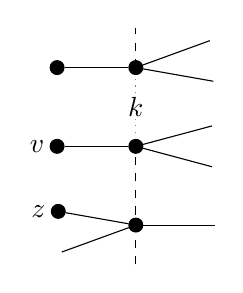
\begin{tikzpicture}[
                    nodes={draw, circle, fill=black, inner sep=0, minimum size=5pt},
                    label distance=1pt]
                \node (2) at (0,2) {};
                \node (1) at (0,1) {};
                \node (0) at (0,0) {};
                \draw [dashed] (0,-0.5) -- (0,1);
                \draw [dotted, opacity=0.5] (0,1) -- (0,2);
                \draw [dashed] (0,2) -- (0,2.5);
                \node (_) [draw=none, fill=white] at (0,1.5) {$k$};

                \path (2) ++(180:1cm) node (_) {} edge (2);
                \path (1) ++(180:1cm) node [label={180:$v$}] (_) {} edge (1);
                \path (0) ++(170:1cm) node [label={180:$z$}] (_) {} edge (0);
                \path (0) ++(200:1cm) edge (0);

                \path (2) ++( 20:1cm) edge (2);
                \path (2) ++(-10:1cm) edge (2);
                \path (1) ++( 15:1cm) edge (1);
                \path (1) ++(-15:1cm) edge (1);
                \path (0) ++(  0:1cm) edge (0);
            \end{tikzpicture}
            \caption{}
            \label{fig:lemma case 5}
        \end{minipage}
        \hfill
        \begin{minipage}{0.32\textwidth}
            \centering
            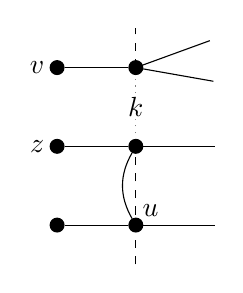
\begin{tikzpicture}[
                    nodes={draw, circle, fill=black, inner sep=0, minimum size=5pt},
                    label distance=1pt]
                \node (2) at (0,2) {};
                \node (1) at (0,1) {};
                \node (0) [label={45:$u$}] at (0,0) {};
                \draw [dashed] (0,-0.5) -- (0,1);
                \draw [dotted, opacity=0.5] (0,1) -- (0,2);
                \draw [dashed] (0,2) -- (0,2.5);
                \node (_) [draw=none, fill=white] at (0,1.5) {$k$};

                \path (2) ++(180:1cm) node [label={180:$v$}] (_) {} edge (2);
                \path (1) ++(180:1cm) node [label={180:$z$}] (_) {} edge (1);
                \path (0) ++(180:1cm) node (_) {} edge (0);

                \path (2) ++( 20:1cm) edge (2);
                \path (2) ++(-10:1cm) edge (2);
                \path (1) ++(  0:1cm) edge (1);
                \path (0) ++(  0:1cm) edge (0);
                \path (0) edge [bend left] (1);
            \end{tikzpicture}
            \caption{}
            \label{fig:lemma case 6}
        \end{minipage}
    \end{figure}
    Now suppose at most five of the edges incident to the separation go to one side, and we have
    two cases: if we have Figure \ref{fig:lemma case 4}, then $\{u,v\}$ is a 2-separation of
    $G^\prime$ (regardless of whether $v=z$), a contradiction; and if we have Figure
    \ref{fig:lemma case 5}, then the face $k$ is a big face (regardless of whether $v=z$).
    Now suppose at most four of the edges incident to the separation go to one side, then we have
    Figure \ref{fig:lemma case 6}, in which case if $v=z$ then $\{u,v\}$ is a 2-separation, but if
    $v\neq z$, then the face $k$ is a big face.

    Since $G^{\prime\prime}$ is 4-connected and planar, then a result in \cite{Tutte1956-dq} says
    that it is Hamiltonian.
    By construction, we know that every way a Hamiltonian cycle in $G^{\prime\prime}$ can pass
    through a vertex in $V(G^{\prime\prime})\setminus V(G^\prime)$ can be replaced with an edge in
    the same face of $G^\prime$, so construct a Hamiltonian graph $H$ in which we do just that.
    \begin{figure}
        \centering
        \begin{tikzpicture}[
                nodes={draw, circle, fill=black, inner sep=0, minimum size=5pt},
                label distance=1pt]
            \node (1) at (0,0) {};
            \path (1) ++( 30:15mm) edge [dashed] (1);
            \path (1) ++( 90:15mm) edge (1);
            \path (1) ++(150:15mm) edge [dashed] (1);
            \path (1) ++(210:15mm) edge (1);
            \path (1) ++(270:15mm) edge [dashed] (1);
            \path (1) ++(330:15mm) edge (1);

            \draw [->, very thick] (3.5,0) -- (4.5,0);

            \node (a) at (8,0) {};
            \path (a) ++( 30: 7mm) node (b) {};
            \path (a) ++( 90:10mm) node (c) {};
            \path (a) ++(150: 7mm) node (d) {};
            \path (a) ++(210:10mm) node (e) {};
            \path (a) ++(270: 7mm) node (f) {};
            \path (a) ++(330:10mm) node (g) {};
            \draw (a) -- (b) -- (c) -- (d);
            \draw (a) -- (d) -- (e) -- (f);
            \draw (a) -- (f) -- (g) -- (b);
            \path (c) ++( 15:10mm) edge [dashed] (c);
            \path (c) ++( 90:10mm) edge (c);
            \path (c) ++(165:10mm) edge [dashed] (c);
            \path (e) ++(135:10mm) edge [dashed] (e);
            \path (e) ++(210:10mm) edge (e);
            \path (e) ++(285:10mm) edge [dashed] (e);
            \path (g) ++(255:10mm) edge [dashed] (g);
            \path (g) ++(330:10mm) edge (g);
            \path (g) ++( 45:10mm) edge [dashed] (g);
        \end{tikzpicture}
        \caption{Vertex operation with new edges}
        \label{fig:vertex operation with new edges}
    \end{figure}
    Now consider a vertex of $H$ on which the inverse vertex operation was applied when
    constructing $G^\prime$ from $G$, and apply the transformation depicted in Figure
    \ref{fig:vertex operation with new edges}, where the dashed lines on the left represent edges
    that were possibly added during the construction of $H$.
    Every dashed line on the left side of the figure has two possible positions on the right side,
    and we choose the one which does not overlap with the other edge of the Hamiltonian cycle in
    $H$, therefore, we can extend that Hamiltonian cycle through the construction.
    Repeating this gives us a Hamiltonian graph $H^\prime$ which is just $G$ but with at most one
    edge added to every big face, which completes the proof.
\end{proof}

% With this theorem, we finish this paper with an interesting corollory regarding the double graphs
% of a subset of Barnette graphs.
%
% \begin{corollary}
%     Let $G$ be a Barnette graph.
%     If the dual of $G$ has an orientation in which every vertex of degree at least 6 has in-degree
%     at most 1, then the double graph of $G$ has a cycle on at least $\lvert G\rvert$ vertices.
% \end{corollary}

\bibliographystyle{abbrv}
\bibliography{references}

\end{document}
